\documentclass[]{scrartcl}
\usepackage[utf8]{inputenc}
\usepackage[T1]{fontenc}
\usepackage[T2A]{fontenc}
\usepackage[finnish]{babel}
\usepackage{linguex} 
\usepackage{longtable} 
\usepackage{booktabs}
\usepackage{amsthm}
\usepackage{graphicx}
\newtheorem{maar}{Määritelmä}
\usepackage{fixltx2e} % provides \textsubscript
\usepackage{textcomp} % provides \textsubscript
\usepackage{hyperref}
\usepackage{xcolor}

\providecommand{\tightlist}{%
  \setlength{\itemsep}{0pt}\setlength{\parskip}{0pt}}

\hypersetup{
    colorlinks,
    linkcolor={red!50!black},
    citecolor={blue!50!black},
    urlcolor={blue!80!black}
}
\author{Juho Härme}
\title{Morfologia-kurssin luentomateriaaleja}
\date{\today}
\begin{document}
\maketitle
\tableofcontents
\newpage



\section{Luento 5: sija kieliopillisena kategoriana
2}\label{luento-5-sija-kieliopillisena-kategoriana-2}

\begin{itemize}
\tightlist
\item
  \href{https://mustikka.uta.fi/~juho_harme/morfologia/\#tästä-kurssista}{Takaisin
  sivun ylälaitaan}
\item
  \href{http://mustikka.uta.fi/~juho_harme/morfologia/materiaalit/luento5.pdf}{Lataa
  PDF}
\item
  \href{http://mustikka.uta.fi/~juho_harme/morfologia/presentations/luento5.html}{Tutki
  luentokalvoja}
\item
  \href{http://mustikka.uta.fi/~juho_harme/morfologia/tehtavat/luento5.pdf}{Tutki
  tuntitehtäviä}
\end{itemize}

(Huom: pdf-versiossa wiktionarylinkit eivät toistaiseksi toimi)

Tällä luennolla sijakategoriaa käsitellään vielä taivutusopin kannalta
ja tarkastellaan poikkeuksia edellä esitettyihin deklinaatioihin. Lopuksi pohditaan
sanapainon vaihtelua eri taivutusmuodoissa.

\subsection{Sekamuotoja ja
poikkeuksia}\label{sekamuotoja-ja-poikkeuksia}

Edellä lueteltujen viiden taivutustyypin voi nähdä muodostavan
selkeimmät pääryhmät, joihin suurin osa substantiiveista voidaan
sovittaa. Näiden ulkopuolelle jää kuitenkin väistämättä iso joukko
substantiiveja. Seuraavassa esitetään muutamia huomioita ja
säännönmukaisuuksia näistä sanoista.

\subsubsection{Muutoksia vartaloissa}\label{muutoksia-vartaloissa}

\paragraph{Äänteenmuutokset}\label{uxe4uxe4nteenmuutokset}

\subparagraph{Väistyvä vokaali}\label{vuxe4istyvuxe4-vokaali}

Ehkäpä merkittävin yksittäinen sanojen sijataivutukseen vaikuttava
morfofonologinen ilmiö on niin sanottu väistyvä vokaali (беглый
гласный). Tällä ilmiöllä viitataan lähinnä /о/- ja /э/-vokaalien
vaihteluun nollaäänteen/nollavokaalin (нуль звука/нуль гласного) kanssa.
Katsotaan paria esimerkkiä\footnote{esimerkit
  \href{http://ruscorpora.ru}{kansalliskorpuksesta}}:

\begin{enumerate}
\def\labelenumi{(\arabic{enumi})}
\tightlist
\item
  Световой сигнал выдергивал её из глубокого \textbf{сна}.
\item
  Враждебность к \textbf{иностранцам} в России глубоко обеспокоила его
\item
  ``Два пункта в справочнике, пара-тройка \textbf{статей} в прессе ― это
  и убило Бернара Луазо''
\end{enumerate}

Esimerkkien 1--3 lihavoidut substantiivit ovat kaikki sanoja, joiden
taivutusmuodoissa väistyvän vokaalin ilmiö näkyy. Esimerkiksi
sananmuodon \emph{сна} yksikön nominatiivi on с\textbf{о}н ja
sananmuodon \emph{иностранцам} иностран\textbf{е}ц. Myös sananmuoto
\emph{статьей} osuu väistyvän vokaalin piiriin, vaikkei ensi
silmäykseltä siltä näyttäisikään. Katsotaan ilmiötä tarkemmin
Nikunlassin (2002: 113-114) ja Šeljakinin (2006: 59-60) pohjalta.

Nikunlassin mukaan väistyvälle vokaalille voidaan esittää yksinkertainen
perussääntö: jos sananmuodossa väistyvänä vokaalina ilmenevä foneemi
esiintyy \textbf{ennen nollapäätettä} (ø), se edustuu konkreettisena
vokaalina, muussa tapauksessa nollavokaalina.

Ajatellaan edellä esitetyn pohjalta sanaa \emph{сон} ja katsotaan sen
taivutusparadigmaa (mukana sekä yksikkö että monikko):

\begin{longtable}[c]{@{}lll@{}}
\toprule
Sija & Päätemorfi & esim.\tabularnewline
\midrule
\endhead
y.nom. & ø & сон\tabularnewline
y.gen. & /а/ & сна\tabularnewline
y.akk. & /ø/ \textasciitilde{} /a/ & сон\tabularnewline
y.dat. & /у/ & сну\tabularnewline
y.instr. & /ом/ & cном\tabularnewline
y.prep. & /е/ \textasciitilde{} /и & сне\tabularnewline
------- & --------- & ---\tabularnewline
m.nom. & /и/ & сны\tabularnewline
m.gen. & /ов/ & снов\tabularnewline
m.akk. & /и/ & сны\tabularnewline
m.dat. & /ам/ & снам\tabularnewline
m.instr. & /ами/ & cнами\tabularnewline
m.prep. & /ах/ & снах\tabularnewline
\bottomrule
\end{longtable}

Kuten taulukosta huomataan, ainoa sija, joka edustuu nollapäätteenä, on
yksikön nominatiivi. Edellä esitetyn säännön mukaisesti tällöin myös
väistyvä vokaali esiintyy oikeasti vokaalina, muissa tapauksissa
nollaäänteenä. Šeljakinin (2006: 59) luokittelussa \emph{сон} kuuluu
ensimmäiseen väistyvän vokaalin sisältävien sanojen ryhmään. Edellä
mainittu статья sekä esimerkiksi sanat \emph{ведро}, \emph{окно}
kuuluvat toiseen, jossa ainoa väistyvän vokaalin sisältävä muoto on
monikon genetiivi. Tämä sopii edellä esitettyyn sääntöön: näillä
sanoilla monikon genetiivi esiintyy nimenomaan nollapäätteenä.

Pohdi tarkemmin ilmiötä tutkimalla esimerkiksi seuraavien sanojen
taivutusmuotoja (klikkaamalla linkkiä pääset wikisanakirjan
artikkeliin):

\begin{itemize}
\tightlist
\item
  \href{https://ru.wiktionary.org/wiki/рот}{рот},
  \href{https://ru.wiktionary.org/wiki/сон}{сон},
  \href{https://ru.wiktionary.org/wiki/ров}{ров},
  \href{https://ru.wiktionary.org/wiki/рожь}{рожь},
  \href{https://ru.wiktionary.org/wiki/лоб}{лоб},
  \href{https://ru.wiktionary.org/wiki/мох}{мох},
  \href{https://ru.wiktionary.org/wiki/лед}{лед},
  \href{https://ru.wiktionary.org/wiki/шов}{шов},
  \href{https://ru.wiktionary.org/wiki/день}{день},
  \href{https://ru.wiktionary.org/wiki/лев}{лев},
  \href{https://ru.wiktionary.org/wiki/пень}{пень}
\item
  \href{https://ru.wiktionary.org/wiki/посол}{посол},
  \href{https://ru.wiktionary.org/wiki/орёл}{орёл},
  \href{https://ru.wiktionary.org/wiki/пепел}{пепел},
  \href{https://ru.wiktionary.org/wiki/котёл}{котёл}
\item
  \href{https://ru.wiktionary.org/wiki/висок}{висок},
  \href{https://ru.wiktionary.org/wiki/дружок}{дружок},
\item
  \href{https://ru.wiktionary.org/wiki/локоть}{локоть},
  \href{https://ru.wiktionary.org/wiki/ноготь}{ноготь},
\item
  \href{https://ru.wiktionary.org/wiki/огонь}{огонь},
  \href{https://ru.wiktionary.org/wiki/корень}{корень},
\item
  \href{https://ru.wiktionary.org/wiki/любимец}{любимец},
  \href{https://ru.wiktionary.org/wiki/перец}{перец},
\item
  \href{https://ru.wiktionary.org/wiki/воробей}{воробей},
  \href{https://ru.wiktionary.org/wiki/муравей}{муравей},
  \href{https://ru.wiktionary.org/wiki/ручей}{ручей}
\end{itemize}

Monikon genetiivimuoto \emph{статьей} saattaa vielä hämätä. Miten niin
siinä on väistyvä vokaali? Sanan /статья/ juurimorfi on tarkkaan ottaen
/стать/ eli foneettisessa asussa /статj/ (pehmeä merkki ei merkitse
tässä kohden pelkkää liudennusta -- tähän riittäisi pelkkä
я-kirjainkin). Nollavokaalin sisältävissä muodoissa статья taipuu siis
cтатьи, статьям jne. Monikon genetiivi on kuitenkin nollapäätteinen, eli
muoto olisi ilman väistyvää vokaalia juurimorfi + ø, toisin sanoen
/статj/ + ø. Tähän nollapäätteen edelle livahtaa väistyvä vokaali е,
jolloin muoto on /статej/ø/. Tätä ei tule sekoittaa /ей/-morfeemiin
monikon genetiivin tunnuksena, vaan monikon tunnus on tässä nollapääte
ja vokaali kuuluu juurimorfiin -- se ei vain esiinny nykykielessä sanan
muissa muodoissa.

Kyseessä on siis melko laaja, muttei kuitenkaan automaattinen ilmiö. Se
esiintyy substantiiveilla tiettyjen suffiksien yhteydessä, ei kuitenkaan
aina. Usein väistyvän vokaalin ennustamisessa auttaakin paitsi suffiksi,
myös sanapaino. Esimerkiksi sanat \emph{америкАнец} ja \emph{инострАнец}
sisältävät väistyvän vokaalin, sana близнЕц ei. Sanat \emph{кОрень} ja
\emph{кАмень} sisältävät väistyvän vokaalin, sana \emph{олЕнь} ei.
Lisäksi on todettava, että tiettyjen konsonanttiyhdistelmien läsnä
ollessa nollavokaali ei esiinny, vaikka voisi olettaa: хитрЕц-хитрецА.

\paragraph{Muita
äänteenmuutostapauksia}\label{muita-uxe4uxe4nteenmuutostapauksia}

Väistyvän vokaalin lisäksi myös eräät muut ilmiöt vaikuttavat
substantiivien sijataivutukseen. Näitä ovat esimerkiksi
\emph{х/ш}-vaihtelu ja \emph{к/ч}-vaihtelu: Ухо/Уха mutta Уши/ушЕй -
Око/Ока, mutta Очи/очЕй. Lisäksi sanalla сосед on monikossa liudentunut
vartalo (vrt. yks.gen. соседа - mon.gen соседей). (Nikunlassi 2002:
141).

\paragraph{Yksittäisiä tapauksia}\label{yksittuxe4isiuxe4-tapauksia}

Substantiiveilla мать ja дочь on useimmissa sijamuodoissa poikkeava
vartalo:

\begin{longtable}[c]{@{}lll@{}}
\toprule
Sija & Päätemorfi & esim.1\tabularnewline
\midrule
\endhead
Nom. & /ø/ & мать\tabularnewline
Gen. & /и/ & матери\tabularnewline
Akk. & /ø/ & мать\tabularnewline
Dat. & /и/ & матери\tabularnewline
Instr. & /ju/ & матерью\tabularnewline
Prep. & /и/ & матери\tabularnewline
\bottomrule
\end{longtable}

Toinen huomionarvoinen vartalonmuutosten ryhmään osuva sanajoukko ovat
yhdyssanat tyyppiä \emph{полдень}. Nämä sanat voivat saada ylimääräisen
у-vokaalin: \emph{полубутылки}, \emph{полубутылке} jne. Tästä ilmiöstä
ei kuitenkaan ole mahdollista tehdä yleispätevää sääntöä. Esimerkiksi
Šeljakin(2006: 50) toteaa (korostus minun):

``При изменении по падежам \ldots{} компонент пол \textbf{может
заменяться} компонентом полу''

Jonkinnäköisenä suuntaviivana voinee sanoa, että у-vokaalin sisältävät
muodot ovat usein tyyliltään kirjallisempia.

Isachenko (2003{[}1965{]}: 167) mainitsee vielä esimerkiksi seuraavia
poikkeuksellisesti taipuvia sanoja (linkit vievät wikisanakirjan
artikkeleihin, joista voit tutkia taivutusta tarkemmin):
\href{https://ru.wiktionary.org/wiki/курица}{курица},
\href{https://ru.wiktionary.org/wiki/чудо}{чудо},
\href{https://ru.wiktionary.org/wiki/небо}{небо}
\href{https://ru.wiktionary.org/wiki/судно}{судно}.

Aivan omanlainen poikkeuksensa on sana
\href{https://ru.wiktionary.org/wiki/мечта}{мечта}, jonka monikon
genetiivimuoto on hankala määritellä. Ainoa järkevä ratkaisu on käyttää
muotoa \emph{мечтаний}, jonka voi varsinaisesti nähdä olevan peräisin
sanasta \emph{мечтание}.

\subsubsection{Monikkoon liittyviä
poikkeuksia}\label{monikkoon-liittyviuxe4-poikkeuksia}

Monilla 1. deklinaatioon kuuluvilla sanoilla monikon pääte ei aina ole
odotuksenmukaisesti /и/, vaan tietyissä tapauksissa /а/. Näin on
esimerkiksi seuraavilla sanoilla (täydellinen lista ks. Шелякин 2006:
52--53):

\href{https://ru.wiktionary.org/wiki/бок}{бок},
\href{https://ru.wiktionary.org/wiki/век}{век},
\href{https://ru.wiktionary.org/wiki/глаз}{глаз},
\href{https://ru.wiktionary.org/wiki/дом}{дом},
\href{https://ru.wiktionary.org/wiki/адрес}{адрес},
\href{https://ru.wiktionary.org/wiki/берег}{берег},
\href{https://ru.wiktionary.org/wiki/вечер}{вечер},
\href{https://ru.wiktionary.org/wiki/лагерь}{лагерь},
\href{https://ru.wiktionary.org/wiki/паспорт}{паспорт},
\href{https://ru.wiktionary.org/wiki/профессор}{профессор}

Joillakin substantiiveilla puolestaan on kaksi eri monikkomuotoa, niin
että muodoilla usein on eri merkitys. Tällaisia sanoja ovat esimerkiksi
\emph{образ} (\emph{образы}, `hahmot' - \emph{образА}, `ikonit'),
\emph{пропуск} (\emph{прОпуски}, `poissaolot' - \emph{пропускА},
`pääsyluvat'), \emph{лист} (\emph{листЫ},
`paperit/sivut',\emph{лИстья},`lehdet').

Erityistä huomiota kannattaa kiinnittää sanojen \emph{колено} ja
\emph{яблоко} monikoihin. Sanalla колено on kaksi monikon nominatiivia,
joista toinen (коленА) ei viittaa polviin fysiologisena ilmiönä vaan
esimerkiksi Israelin heimoihin Raamatussa; muoto \emph{колЕни} on se,
joka viittaa колено-sanaan sen tutummassa merkityksessä. Яблоко-sana
muistuttaa taivutukseltaan колено-sanaa siinä mielessä, että sekin
noudattaa muuten neljättä deklinaatiota, mutta monikon nominatiivi ei
osukaan edellä monikon kolmanneksi deklinaatioksi määriteltyyn ryhmään
vaan ilmaistaan /и/-morfilla.

\subsubsection{Sekadeklinaatioita}\label{sekadeklinaatioita}

Tietyt sukunimet taipuvat muuten 1. deklinaation mukaan, mutta niiden
yksikön instrumentaalimuoto muistuttaa adjektiivien
instrumentaalimuotoa:

\begin{longtable}[c]{@{}llll@{}}
\toprule
Sija & Päätemorfi & esim. 1 & esim.2\tabularnewline
\midrule
\endhead
Nom. & /ø/ & Иванов & Малкин\tabularnewline
Gen. & /а/ & Иванова & Малкина\tabularnewline
Akk. & /а/ & Иванова & Малкина\tabularnewline
Dat. & /у/ & Иванову & Малкину\tabularnewline
Instr. & /ым/ & Ивановым & Малкиным\tabularnewline
Prep. & /е/ & Иванове & Малкине\tabularnewline
\bottomrule
\end{longtable}

Kuitenkin esimerkiksi ук-päätteiset sukunimet saavat normaalin yksikön
instrumentaalin päätteen:

\begin{enumerate}
\def\labelenumi{(\arabic{enumi})}
\setcounter{enumi}{3}
\tightlist
\item
  фильм с Малкиным и Ковальчуком
\end{enumerate}

Toinen esimerkki sekadeklinaatiosta on sana
\href{https://ru.wiktionary.org/wiki/путь}{путь}, jossa sekoittuvat
ensimmäisen ja kolmannen deklinaation päätteet siten, että
instrumentaalin pääte on ensimmäisen deklinaation mukainen, genetiivi,
datiivi ja prepositionaali kolmannen. Vertailun vuoksi alla on kuvattu
myös yksi substantiivi kummastakin varsinaisesta deklinaatiotyypistä:

\begin{longtable}[c]{@{}lll@{}}
\toprule
Sija & Päätemorfi & esim 1.\tabularnewline
\midrule
\endhead
Nom. & /ø/ & путь\tabularnewline
Gen. & /и/ & пути\tabularnewline
Akk. & /ø/ & путь\tabularnewline
Dat. & /и/ & пути\tabularnewline
Instr. & /ом/ & путём\tabularnewline
Prep. & /и/ & пути\tabularnewline
\bottomrule
\end{longtable}

\subsection{Deklinaatioista ja
painotyypeistä}\label{deklinaatioista-ja-painotyypeistuxe4}

Aleksandr Isatšenko toteaa laajassa venäjän kieliopin kuvauksessaan
seuraavasti (2003{[}1965{]}: 129):

\emph{Морфологическая характеристика имен существительных в русском
языке не ограничивается указанием всех падежных окончаний. Чтобы
правильно пользоваться словом, необходимо усвоить его акцентологические
особенности.}

Vapaan sanapainon takia olennaista venäjän substantiivien morfologiassa
on paitsi päätteiden tunteminen, myös sen tiedostaminen, että eri
sananmuotojen ääntämys vaihtelee painon osalta ja myös painon suhteen
sanoja voidaan jossain määrin ryhmitellä.

Tässä yhteydessä ei luennoilla ehditä tekemään erityisen kattavaa
katsausta eri painotyyppeihin, vaan tarkempi tutustuminen
painotyyppeihin jää itsenäisen opiskelun varaan.

Käytännössä sanapainoa pohdittaessa on kaksi vaihtoehtoa: joko paino
sijaitsee vartalolla tai päätteellä. Eri painotyypit voidaan hahmottaa
tämän opposition valossa niin, että tyypit erottaa toisistaan se, missä
muodoissa paino on päätteellä, missä taas vartalolla. Usein yksikkö ja
monikko muodostavat selkeän jakolinjan, mutta myös yksittäiset sijat
voivat erottua joukosta. Merkittävä jakolinja kulkee nominatiivin ja
\emph{obliikvisijojen} (косвенные падежи) välillä: usein esimerkiksi
poikkeava monikon taivutusmuoto on juuri nominatiivi.

Itse asiassa hivenen yksinkertaistaen substantiivien sanapainon
vaihtelun voi typistää seuraavaan L.L. Kasatkinin (2006: 68) esittämään
taulukkoon:

\begin{figure}[htbp]
\centering
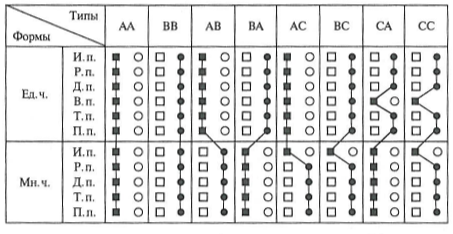
\includegraphics{kasatkin.png}
\caption{}
\end{figure}

Taulukossa neliöt merkitsevät sanavartaloa, ympyrät päätettä. Musta
neliö tai ympyrä tarkoittaa painon sijaintia. Taulukko listaa tavalliset
kahdeksan painotyyppiä ja osoittaa painon vaihtelun säännönmukaisuuden.
Siihen kannattaa palata, kun käyt läpi seuraavassa esitettyjä
deklinaatiokohtaisia painotyyppejä. Tarkasteluni perustuu Isatšenkon
(2003{[}1965{]}: 130--136, 141--143, 152--156, 161) esitykseen.

\subsubsection{I deklinaation
painotyypit}\label{i-deklinaation-painotyypit}

Ensimmäisen deklinaation sanoille voidaan erottaa viisi painotyyppiä,
joita nimitän tässä seuraavasti:

\begin{enumerate}
\def\labelenumi{\arabic{enumi}.}
\tightlist
\item
  завОд-tyyppi
\item
  стол-tyyppi
\item
  нос-tyyppi
\item
  волк-tyyppi
\end{enumerate}

\paragraph{ЗавОд-tyyppi}\label{ux437ux430ux432ux43eux434-tyyppi}

ЗавОд-tyypin sanoissa paino on niin yksikössä kuin monikossa vartalolla:

\begin{longtable}[c]{@{}lll@{}}
\toprule
sija & yks. & mon.\tabularnewline
\midrule
\endhead
nom. & завОд & завОды\tabularnewline
gen. & завОда & завОдов\tabularnewline
dat. & завОду & завОдам\tabularnewline
akk. & завОд & завОды\tabularnewline
instr. & завОдом & завОдами\tabularnewline
prep. & завОде & завОдах\tabularnewline
\bottomrule
\end{longtable}

Tähän tyyppiin kuuluu suuri osa maskuliineista. Joukossa on

\begin{enumerate}
\def\labelenumi{\arabic{enumi}.}
\tightlist
\item
  \textbf{johtamattomia (непроизводные) sanoja} kuten
  \href{http://ru.wiktionary.org/wiki/баран}{барАн},
  \href{http://ru.wiktionary.org/wiki/стул}{стул},
  \href{http://ru.wiktionary.org/wiki/народ}{нарОд},
  \href{http://ru.wiktionary.org/wiki/союз}{соЮз},
  \href{http://ru.wiktionary.org/wiki/закон}{закОн}.
\item
  paljon \textbf{johdettuja (производные)}
  \href{http://ru.wiktionary.org/wiki/начальник}{начАльник},
  \href{http://ru.wiktionary.org/wiki/грохот}{грОхот},
  \href{http://ru.wiktionary.org/wiki/заработок}{зАработок},
  \href{http://ru.wiktionary.org/wiki/отдел}{отдЕл},\href{http://ru.wiktionary.org/wiki/подоконник}{подокОнник}
\item
  melko uusia \textbf{lainoja}:
  \href{http://ru.wiktionary.org/wiki/чемодан}{чемодАн},
  \href{http://ru.wiktionary.org/wiki/билет}{билЕт},
  \href{http://ru.wiktionary.org/wiki/магазин}{магазИн},\href{http://ru.wiktionary.org/wiki/трамвай}{трамвАй}
\item
  \textbf{erisnimiä} ИвАн, НиколАй, БетхОвен, ДунАй
\end{enumerate}

\paragraph{Стол-tyyppi}\label{ux441ux442ux43eux43b-tyyppi}

Стол-tyypin sanoilla paino on yksikön nominatiivissa (ja akkusatiivissa)
teknisesti ottaen vartalolla (usein suffiksilla, kuten -ец), kaikissa
muissa muodoissa päätteellä. Käytännössä tuloksena on paradigma, jossa
paino on aina viimeisellä tavulla:

\begin{longtable}[c]{@{}lll@{}}
\toprule
sija & yks. & mon.\tabularnewline
\midrule
\endhead
nom. & стОл & столЫ\tabularnewline
gen. & столА & столОв\tabularnewline
dat. & столУ & столАм\tabularnewline
akk. & стол & столЫ\tabularnewline
instr. & столОм & столАми\tabularnewline
prep. & столЕ & столАх\tabularnewline
\bottomrule
\end{longtable}

Tähän tyyppiin kuuluu monia \textbf{johtamattomia yksitavuisia sanoja}:
бык, вол, вождь,
врач,гриб,гроб,двор,дождь,ёж,карандаш,пирог,рубль,чердак.

Johdettujen sanojen osalta voidaan erottaa koko joukko suffikseja, jotka
tuottavat tämän painotyypin substantiivin:

\begin{itemize}
\tightlist
\item
  ец: \href{http://ru.wiktionary.org/wiki/певец}{певЕц},
  \href{http://ru.wiktionary.org/wiki/купец}{купЕц},
  \href{http://ru.wiktionary.org/wiki/глупец}{глупЕц}

  \begin{itemize}
  \tightlist
  \item
    Myös sanat, joissa ец ei enää nykykielen kannalta suffiksi:
    \href{http://ru.wiktionary.org/wiki/отец}{отЕц},
    \href{http://ru.wiktionary.org/wiki/конец}{конЕц},\href{http://ru.wiktionary.org/wiki/песец}{песЕц}
  \end{itemize}
\item
  ик: \href{http://ru.wiktionary.org/wiki/ученик}{ученИк},
  \href{http://ru.wiktionary.org/wiki/грузовик}{грузовИк},
  \href{http://ru.wiktionary.org/wiki/большевик}{большевИк},
  \href{http://ru.wiktionary.org/wiki/старик}{старИк},\href{http://ru.wiktionary.org/wiki/двойник}{двойнИк}
\item
  ак:
  \href{http://ru.wiktionary.org/wiki/рыбак}{рыбАк},\href{http://ru.wiktionary.org/wiki/дурак}{дурАк}\href{http://ru.wiktionary.org/wiki/казак}{казАк},
\item
  як: \href{http://ru.wiktionary.org/wiki/земляк}{землЯк},
  \href{http://ru.wiktionary.org/wiki/поляк}{полЯк},\href{http://ru.wiktionary.org/wiki/коньяк}{коньЯк}
\item
  ок: \href{http://ru.wiktionary.org/wiki/воротничок}{воротничОк},
  \href{http://ru.wiktionary.org/wiki/белок}{белОк},
  \href{http://ru.wiktionary.org/wiki/песок}{песОк},\href{http://ru.wiktionary.org/wiki/потолок}{потолОк}
\item
  ун:
  \href{http://ru.wiktionary.org/wiki/хвастун}{хвастУн},\href{http://ru.wiktionary.org/wiki/бегун}{бегУн}
\item
  \href{http://ru.wiktionary.org/wiki/ух}{ух}:
  \href{http://ru.wiktionary.org/wiki/петух}{петУх},\href{http://ru.wiktionary.org/wiki/пастух}{пастУх}
\item
  \href{http://ru.wiktionary.org/wiki/ач}{ач}:
  \href{http://ru.wiktionary.org/wiki/скрипач}{скрипАч},
  \href{http://ru.wiktionary.org/wiki/силач}{силАч},\href{http://ru.wiktionary.org/wiki/трубач}{трубАч}
\item
  ич: ИльИч, кирпИч
\end{itemize}

\paragraph{Нос-tyyppi}\label{ux43dux43eux441-tyyppi}

Нос-tyypissä paino on yksikössä vartalolla, monikossa päätteellä:

\begin{longtable}[c]{@{}lll@{}}
\toprule
sija & yks. & mon.\tabularnewline
\midrule
\endhead
nom. & нОс & носЫ\tabularnewline
gen. & нОса & носОв\tabularnewline
dat. & нОсу & носАм\tabularnewline
akk. & нОс & носЫ\tabularnewline
instr. & нОсом & носАми\tabularnewline
prep. & о нОсе & о носАх\tabularnewline
\bottomrule
\end{longtable}

Tähän tyyppiin kuuluvat muun muassa seuraavat pääosin yksitavuiset
sanat:

\href{http://ru.wiktionary.org/wiki/альт}{альт},
\href{http://ru.wiktionary.org/wiki/бал}{бал},
\href{http://ru.wiktionary.org/wiki/бас}{бас},
\href{http://ru.wiktionary.org/wiki/борт}{борт},
\href{http://ru.wiktionary.org/wiki/бунт}{бунт},
\href{http://ru.wiktionary.org/wiki/вал}{вал},
\href{http://ru.wiktionary.org/wiki/верх}{верх},
\href{http://ru.wiktionary.org/wiki/воз}{воз},
\href{http://ru.wiktionary.org/wiki/год}{год},
\href{http://ru.wiktionary.org/wiki/гроб}{гроб},
\href{http://ru.wiktionary.org/wiki/долг}{долг},
\href{http://ru.wiktionary.org/wiki/жир}{жир},
\href{http://ru.wiktionary.org/wiki/круг}{круг},
\href{http://ru.wiktionary.org/wiki/лад}{лад},
\href{http://ru.wiktionary.org/wiki/мозг}{мозг},
\href{http://ru.wiktionary.org/wiki/мост}{мост},
\href{http://ru.wiktionary.org/wiki/низ}{низ},
\href{http://ru.wiktionary.org/wiki/нос}{нос},
\href{http://ru.wiktionary.org/wiki/пан}{пан},
\href{http://ru.wiktionary.org/wiki/пар}{пар},
\href{http://ru.wiktionary.org/wiki/пир}{пир},
\href{http://ru.wiktionary.org/wiki/плуг}{плуг},
\href{http://ru.wiktionary.org/wiki/раз}{раз},
\href{http://ru.wiktionary.org/wiki/ряд}{ряд},
\href{http://ru.wiktionary.org/wiki/сад}{сад},
\href{http://ru.wiktionary.org/wiki/суп}{суп},
\href{http://ru.wiktionary.org/wiki/сыр}{сыр},
\href{http://ru.wiktionary.org/wiki/шаг}{шаг},
\href{http://ru.wiktionary.org/wiki/шкаф}{шкаф},
\href{http://ru.wiktionary.org/wiki/торг}{торг},
\href{http://ru.wiktionary.org/wiki/чай}{чай}

Kannattaa huomata, että lähes kaikilla näistä sanoista on olemassa
у-päätteinen lokatiivimuoto: на носУ, в рядУ jne.

Oman ryhmänsä tämän painotyypin sisällä muodostavat sanat, joilla on
epäsäännöllinen /а/-päätteinen monikon nominatiivi:
\href{http://ru.wiktionary.org/wiki/берег}{берег},
\href{http://ru.wiktionary.org/wiki/глаз}{глаз},
\href{http://ru.wiktionary.org/wiki/голос}{голос},
\href{http://ru.wiktionary.org/wiki/холож}{холож},
\href{http://ru.wiktionary.org/wiki/друг}{друг},
\href{http://ru.wiktionary.org/wiki/князь}{князь}.

\paragraph{Волк-tyyppi}\label{ux432ux43eux43bux43a-tyyppi}

Волк-tyypin sanoilla paino on vartalolla yksikössä sekä monikon
nominatiivi-/akkusatiivimuodoilla, muuten päätteellä:

\begin{longtable}[c]{@{}lll@{}}
\toprule
sija & yks. & mon.\tabularnewline
\midrule
\endhead
nom. & вОлк & вОлки\tabularnewline
gen. & вОлка & волкОв\tabularnewline
dat. & вОлку & волкАм\tabularnewline
akk. & вОлка & волкОв\tabularnewline
instr. & вОлком & волкАми\tabularnewline
prep. & вОлке & волкАх\tabularnewline
\bottomrule
\end{longtable}

Tähän ryhmään kuuluu lähinnä vanhoja kantavenäläisiä sanoja: бог, ветер,
вОлос, \href{http://ru.wiktionary.org/wiki/вор}{вор},
\href{http://ru.wiktionary.org/wiki/гость}{гость},
\href{http://ru.wiktionary.org/wiki/голубь}{гОлубь},
\href{http://ru.wiktionary.org/wiki/гром}{гром},
\href{http://ru.wiktionary.org/wiki/гусь}{гусь},
\href{http://ru.wiktionary.org/wiki/зверь}{зверь},
\href{http://ru.wiktionary.org/wiki/зуб}{зуб},
\href{http://ru.wiktionary.org/wiki/камень}{камень},
\href{http://ru.wiktionary.org/wiki/корень}{кОрень},
\href{http://ru.wiktionary.org/wiki/лебедь}{лЕбедь},
\href{http://ru.wiktionary.org/wiki/лосось}{лОсось},
\href{http://ru.wiktionary.org/wiki/локоть}{лОкоть},
\href{http://ru.wiktionary.org/wiki/медведь}{медведь},
\href{http://ru.wiktionary.org/wiki/окунь}{Окунь},
\href{http://ru.wiktionary.org/wiki/хлеб}{хлеб},
\href{http://ru.wiktionary.org/wiki/чёрт}{чёрт},
\href{http://ru.wiktionary.org/wiki/уголь}{уголь}.

\subsubsection{II deklinaation
painotyypit}\label{ii-deklinaation-painotyypit}

Toinen deklinaatio on sanapainon kannalta ehkä kielrnoppijalle kaikkein
haastavin, sillä paino ei läheskään aina noudattele kaavaa, jossa
yksikkö ja monikko olisivat johdonmukaisia kokonaisuuksia. Toisen
deklinaation sanat voidaan painon perusteella jakaa seuraaviin kolmeen
pääryhmään:

\begin{enumerate}
\def\labelenumi{\arabic{enumi}.}
\tightlist
\item
  шкОла-tyyppi
\item
  Sanat, joilla yksikössä aina paino päätteellä
\item
  Sanat, joissa yksikön akkusatiivi muodostaa poikkeuksen
\end{enumerate}

Toinen pääryhmä voidaan edelleen jakaa kolmeen alaryhmään:

\begin{enumerate}
\def\labelenumi{\alph{enumi})}
\tightlist
\item
  травА-tyyppi
\item
  свечА-tyyppi
\item
  волнА-tyyppi
\end{enumerate}

Kolmannesta pääryhmästä voidaan erottaa alaluokat:

\begin{enumerate}
\def\labelenumi{\alph{enumi})}
\tightlist
\item
  рукА/головА-tyyppi
\item
  ценА-tyyppi
\end{enumerate}

Mainittujen pääryhmien ulkopuolelle jäävät muun muassa sanat
\href{http://ru.wiktionary.org/wiki/деревня}{дерЕвня} sekä
\href{http://ru.wiktionary.org/wiki/доля}{дОля}.

\paragraph{ШкОла-tyyppi}\label{ux448ux43aux43eux43bux430-tyyppi}

Tavallisin ja produktiivisin toisen deklinaation tyypeistä on
школа-tyyppi, jonka sanoilla paino on muuttumattomasti aina vartalolla:

\begin{longtable}[c]{@{}lll@{}}
\toprule
sija & yks. & mon.\tabularnewline
\midrule
\endhead
nom. & шкОла & шкОлы\tabularnewline
gen. & шкОлы & шкОл\tabularnewline
dat. & шкОле & шкОлам\tabularnewline
akk. & шкОлу & шкОлы\tabularnewline
instr. & шкОлой & шкОлами\tabularnewline
prep. & шкОле & шкОлах\tabularnewline
\bottomrule
\end{longtable}

Joukosta voi erottaa omiksi ryhmikseen:

\begin{enumerate}
\def\labelenumi{\arabic{enumi}.}
\tightlist
\item
  \textbf{johtamattomat} sanat:
  \href{http://ru.wiktionary.org/wiki/кожа}{кОжа},
  \href{http://ru.wiktionary.org/wiki/муха}{мУха},
  \href{http://ru.wiktionary.org/wiki/воля}{вОля},
  \href{http://ru.wiktionary.org/wiki/липа}{лИпа},
  \href{http://ru.wiktionary.org/wiki/репа}{рЕпа},
  \href{http://ru.wiktionary.org/wiki/вера}{вЕра},
  \href{http://ru.wiktionary.org/wiki/лопата}{лопАта},
  \href{http://ru.wiktionary.org/wiki/неделя}{недЕля}
\item
  \textbf{nykykielen kannalta johtamattomat} sanat:
  \href{http://ru.wiktionary.org/wiki/ложка}{лОжка},
  \href{http://ru.wiktionary.org/wiki/свадьба}{свАдьба},
  \href{http://ru.wiktionary.org/wiki/печка}{пЕчка},\href{http://ru.wiktionary.org/wiki/ножка}{нОжка}
\item
  \textbf{lainat}:
  \href{http://ru.wiktionary.org/wiki/фабрика}{фабрика},
  \href{http://ru.wiktionary.org/wiki/кафедра}{кАфедра},
  \href{http://ru.wiktionary.org/wiki/культура}{культУра},
  \href{http://ru.wiktionary.org/wiki/газета}{газЕта},
  \href{http://ru.wiktionary.org/wiki/система}{систЕма},
  \href{http://ru.wiktionary.org/wiki/полемика}{полЕмика}
\end{enumerate}

\paragraph{Sanat, joilla yksikössä paino aina
päätteellä}\label{sanat-joilla-yksikuxf6ssuxe4-paino-aina-puxe4uxe4tteelluxe4}

Kuten edellä todettiin, tämä joukko on mielekästä jakaa kolmeen
alaryhmään, joita kaikkia yhdistää se, että kaikissa yksikön muodoissa
paino on päätteellä mutta jotka eroavat sen perusteella, miten monikon
painot asettuvat. Nämä tyypt eivät ole yhtä yleisiä kuin edellä mainittu
школа-tyyppi, mutta niihin kuuluvat sanat ovat hyvin tavallisia.

\subparagraph{ТравА-tyypin
sanat}\label{ux442ux440ux430ux432ux430-tyypin-sanat}

ТравА-tyypin sanoilla monikon paino on aina vartalolla:

\begin{longtable}[c]{@{}lll@{}}
\toprule
sija & yks. & mon.\tabularnewline
\midrule
\endhead
nom. & травА & трАвы\tabularnewline
gen. & травЫ & трАв\tabularnewline
dat. & травЕ & трАвам\tabularnewline
akk. & травУ & трАвы\tabularnewline
instr. & травОй & трАвами\tabularnewline
prep. & травЕ & трАвах\tabularnewline
\bottomrule
\end{longtable}

Tähän tyyppiin kuuluvat muun muassa seuraavat kaksitavuiset sanat:
\href{http://ru.wiktionary.org/wiki/беда}{бедА},
\href{http://ru.wiktionary.org/wiki/вдова}{вдовА},
\href{http://ru.wiktionary.org/wiki/весна}{веснА},
\href{http://ru.wiktionary.org/wiki/ветла}{ветлА},
\href{http://ru.wiktionary.org/wiki/вина}{винА},
\href{http://ru.wiktionary.org/wiki/война}{войнА},
\href{http://ru.wiktionary.org/wiki/глава}{главА},
\href{http://ru.wiktionary.org/wiki/гряда}{грядА},
\href{http://ru.wiktionary.org/wiki/дыра}{дырА},
\href{http://ru.wiktionary.org/wiki/жена}{женА},
\href{http://ru.wiktionary.org/wiki/звезда}{звездА},
\href{http://ru.wiktionary.org/wiki/змея}{змеЯ},
\href{http://ru.wiktionary.org/wiki/игла}{иглА},
\href{http://ru.wiktionary.org/wiki/игра}{игрА},
\href{http://ru.wiktionary.org/wiki/икра}{икрА},
\href{http://ru.wiktionary.org/wiki/коза}{козА}.
\href{http://ru.wiktionary.org/wiki/луна}{лунА},
\href{http://ru.wiktionary.org/wiki/нора}{норА},
\href{http://ru.wiktionary.org/wiki/нужда}{нуждА},
\href{http://ru.wiktionary.org/wiki/овца}{овцА},
\href{http://ru.wiktionary.org/wiki/оса}{осА},
\href{http://ru.wiktionary.org/wiki/пила}{пилА},\href{http://ru.wiktionary.org/wiki/пчела}{пчелА},\href{http://ru.wiktionary.org/wiki/руда}{рудА},
\href{http://ru.wiktionary.org/wiki/свинья}{свиньЯ},
\href{http://ru.wiktionary.org/wiki/семья}{семьЯ},
\href{http://ru.wiktionary.org/wiki/скала}{скалА},
\href{http://ru.wiktionary.org/wiki/сестра}{сестрА},
\href{http://ru.wiktionary.org/wiki/смола}{смолА},
\href{http://ru.wiktionary.org/wiki/сова}{совА},
\href{http://ru.wiktionary.org/wiki/сосна}{соснА},
\href{http://ru.wiktionary.org/wiki/стрела}{стрелА},
\href{http://ru.wiktionary.org/wiki/струна}{струнА},
\href{http://ru.wiktionary.org/wiki/страна}{странА},\href{http://ru.wiktionary.org/wiki/труба}{трубА}

Lisäksi seuraavia kolmitavuisia ота-päätteisiä:
\href{http://ru.wiktionary.org/wiki/кислота}{кислотА},
\href{http://ru.wiktionary.org/wiki/красота}{красотА},
\href{http://ru.wiktionary.org/wiki/высота}{высотА},
\href{http://ru.wiktionary.org/wiki/сирота}{сиротА},
\href{http://ru.wiktionary.org/wiki/колбаса}{колбасА}.

\subparagraph{свечА-tyyppi}\label{ux441ux432ux435ux447ux430-tyyppi}

СвечА-tyypin monikon paino on obliikvisijoissa päätteellä:

\begin{longtable}[c]{@{}lll@{}}
\toprule
sija & yks. & mon.\tabularnewline
\midrule
\endhead
nom. & свечА & свЕчы\tabularnewline
gen. & свечЫ & свеч\tabularnewline
dat. & свечЕ & свечАм\tabularnewline
akk. & свечУ & свЕчи\tabularnewline
instr. & свечОй & свечАми\tabularnewline
prep. & свечЕ & свечАх\tabularnewline
\bottomrule
\end{longtable}

Tämä tyyppi ei ole yleinen, mutta sisältää esimerkiksi sanat
\href{http://ru.wiktionary.org/wiki/железа}{железА},\href{http://ru.wiktionary.org/wiki/сковорода}{сковородА},
\href{http://ru.wiktionary.org/wiki/строка}{строкА},
\href{http://ru.wiktionary.org/wiki/простыня}{простынЯ}.

\subparagraph{волнА-tyyppi}\label{ux432ux43eux43bux43dux430-tyyppi}

ВолнА-tyypin sanoilla monikon nominatiivin pääte on vartalolla, mutta
obliikvisijoissa on rinnakkaismuotoja (molempi painovaihtoehto
mahdollinen):

\begin{longtable}[c]{@{}lll@{}}
\toprule
sija & yks. & mon.\tabularnewline
\midrule
\endhead
nom. & волнА & вОлны\tabularnewline
gen. & волнЫ & вОлн\tabularnewline
dat. & волнЕ & вОлнам \textasciitilde{} волнАм\tabularnewline
akk. & волнУ & вОлны\tabularnewline
instr. & волнОй & вОлнами \textasciitilde{} волнАми\tabularnewline
prep. & волнЕ & вОлнах \textasciitilde{} волнАх\tabularnewline
\bottomrule
\end{longtable}

Волна-sanan lisäksi tähän harvinaiseen tyyppiin kuuluvat muun muassa
\href{http://ru.wiktionary.org/wiki/дуга}{дугА} (`kaari'),
\href{http://ru.wiktionary.org/wiki/судьба}{судьбА},
\href{http://ru.wiktionary.org/wiki/судья}{судьЯ}.

\paragraph{Sanat, joissa yksikön akkusatiivi muodostaa
poikkeuksen}\label{sanat-joissa-yksikuxf6n-akkusatiivi-muodostaa-poikkeuksen}

Tähän ryhmään kuuluvat sanat ovat monet erittäin tavallisia, ja painon
muuttuminen yksikköparadigman sisällä aiheuttaa kielenoppijan kannalta
paljon epävarmuutta. Tässäkin on kuitenkin kyseessä säännönmukainen
tyyppi, joka on mahdollista opetella. Jaan tyypin tässä kahteen
alaryhmään. Kaikille ryhmille on yhteistä se, että yksikön
akkusatiivissa paino on vartalolla, muissa yksikön muodoissa päätteellä.

\subparagraph{рукА-tyyppi}\label{ux440ux443ux43aux430-tyyppi}

Рука-tyypin sanoilla monikon paino on obliikvisijoissa päätteellä:

\begin{longtable}[c]{@{}lll@{}}
\toprule
sija & yks. & mon.\tabularnewline
\midrule
\endhead
nom. & рукА & рУки\tabularnewline
gen. & руки & рук\tabularnewline
dat. & рукЕ & рукАм\tabularnewline
akk. & рУку & рУки\tabularnewline
instr. & рукОй & рукАми\tabularnewline
prep. & рукЕ & рукАх\tabularnewline
\bottomrule
\end{longtable}

Tähän alatyyppiin voidaan lukea mm. seuraavat:

\href{http://ru.wiktionary.org/wiki/вода}{вода},
\href{http://ru.wiktionary.org/wiki/гора}{гора},
\href{http://ru.wiktionary.org/wiki/доска}{доскА},
\href{http://ru.wiktionary.org/wiki/душа}{душА},
\href{http://ru.wiktionary.org/wiki/зима}{зимА},
\href{http://ru.wiktionary.org/wiki/кроха}{крохА},
\href{http://ru.wiktionary.org/wiki/коса}{косА},
\href{http://ru.wiktionary.org/wiki/река}{рекА},
\href{http://ru.wiktionary.org/wiki/рука}{рукА},
\href{http://ru.wiktionary.org/wiki/зима}{зимА},
\href{http://ru.wiktionary.org/wiki/спина}{спинА},
\href{http://ru.wiktionary.org/wiki/среда}{средА},
\href{http://ru.wiktionary.org/wiki/стена}{стенА},
\href{http://ru.wiktionary.org/wiki/стопа}{стопА},
\href{http://ru.wiktionary.org/wiki/щека}{щекА},
\href{http://ru.wiktionary.org/wiki/нога}{ногА}

Lisäksi samalla tavoin taipuvat eräät useampitavuiset sanat, kuten
\href{http://ru.wiktionary.org/wiki/голова}{голова}:

\begin{longtable}[c]{@{}lll@{}}
\toprule
sija & yks. & mon.\tabularnewline
\midrule
\endhead
nom. & головА & гОловы\tabularnewline
gen. & головЫ & голОв\tabularnewline
dat. & головЕ & головАм\tabularnewline
akk. & гОлову & гОловы\tabularnewline
instr. & головОй & головАми\tabularnewline
prep. & головЕ & головАх\tabularnewline
\bottomrule
\end{longtable}

\subparagraph{цена-tyyppi}\label{ux446ux435ux43dux430-tyyppi}

Tämän alatyypin sanoissa koko monikon paradigma saa painon vartalolle
(joka genetiivin osalta tosin tarkoittaa väistyvän vokaalin tapauksessa
viimeistä tavua):

\begin{longtable}[c]{@{}lll@{}}
\toprule
sija & yks. & mon.\tabularnewline
\midrule
\endhead
nom. & землЯ & зЕмли\tabularnewline
gen. & землИ & земЕль\tabularnewline
dat. & землЕ & зЕмлям\tabularnewline
akk. & зЕмлу & зЕмли\tabularnewline
instr. & землЁй & зЕмлями\tabularnewline
prep. & землЕ & зЕмлях\tabularnewline
\bottomrule
\end{longtable}

Tyyppi on harvalukuinen, sen tavallisimpia sanoja ovat
\href{http://ru.wiktionary.org/wiki/цена}{ценА},
\href{http://ru.wiktionary.org/wiki/земля}{землЯ},
\href{http://ru.wiktionary.org/wiki/изба}{избА} (`pieni mökki').

\subsubsection{III deklinaation
painotyyppejä}\label{iii-deklinaation-painotyyppejuxe4}

Kolmas deklinaatio voidaan jakaa kahteen pääryhmään:

\begin{enumerate}
\def\labelenumi{\arabic{enumi}.}
\tightlist
\item
  Тетрадь-tyyppi
\item
  Вещь-tyyppi
\end{enumerate}

\paragraph{тетрадь-tyyppi}\label{ux442ux435ux442ux440ux430ux434ux44c-tyyppi}

Тертрадь-tyyppi on produktiivinen ja yleinen. Paino lankeaa kaikissa
muodoissa vartalolle:

\begin{longtable}[c]{@{}lll@{}}
\toprule
sija & yks. & mon.\tabularnewline
\midrule
\endhead
nom. & тетрАдь & тетрАди\tabularnewline
gen. & тетрАди & тетрАдей\tabularnewline
dat. & тетрАди & тетрАдям\tabularnewline
akk. & тетрАдь & тетрАди\tabularnewline
instr. & тетрАдью & тетрАдями\tabularnewline
prep. & тетрАди & тетрАдях\tabularnewline
\bottomrule
\end{longtable}

Tyyppiin kuuluu suuri joukko sanoja, jotka voi jakaa karkeasti
seuraaviin alaryhmiin:

\begin{enumerate}
\def\labelenumi{\arabic{enumi}.}
\tightlist
\item
  Yksitavuisia: \href{http://ru.wiktionary.org/wiki/жизнь}{жизнь},
  \href{http://ru.wiktionary.org/wiki/жесть}{жесть},
  \href{http://ru.wiktionary.org/wiki/сталь}{сталь},
  \href{http://ru.wiktionary.org/wiki/шерсть}{шерсть},
  \href{http://ru.wiktionary.org/wiki/нефть}{нефть},
\item
  Kaksitavuisia: \href{http://ru.wiktionary.org/wiki/ладонь}{ладОнь},
  \href{http://ru.wiktionary.org/wiki/кровать}{кровАть},
  \href{http://ru.wiktionary.org/wiki/постель}{постЕль},
  \href{http://ru.wiktionary.org/wiki/прелесть}{прЕлесть},
  \href{http://ru.wiktionary.org/wiki/память}{пАмять},\href{http://ru.wiktionary.org/wiki/помощь}{пОмощь}
\item
  Suurin osa
  \href{http://ru.wiktionary.org/wiki/ость}{ость}-päätteisistä kuuluu
  tähän tyyppiin (näillä yleensä ei monikkomuotoja):
  \href{http://ru.wiktionary.org/wiki/радость}{рАдость},
  \href{http://ru.wiktionary.org/wiki/глупость}{глУпость},\href{http://ru.wiktionary.org/wiki/неожиданность}{неожИданность}
\item
  Vierasperäisiä: \href{http://ru.wiktionary.org/wiki/мораль}{морАль},
  \href{http://ru.wiktionary.org/wiki/медаль}{медАль},
  \href{http://ru.wiktionary.org/wiki/форель}{форЕль},
  \href{http://ru.wiktionary.org/wiki/панель}{панЕль}
\end{enumerate}

\paragraph{вещь-tyyppi}\label{ux432ux435ux449ux44c-tyyppi}

Вещь-tyyppiin kuuluvat III deklinaation sanat, joissa monikon
obliikvisijoissa paino lankeaa päätteelle:

\begin{longtable}[c]{@{}lll@{}}
\toprule
sija & yks. & mon.\tabularnewline
\midrule
\endhead
nom. & вЕщь & вЕщи\tabularnewline
gen. & вЕщи & вещЕй\tabularnewline
dat. & вЕщи & вещАм\tabularnewline
akk. & вЕщь & вЕщи\tabularnewline
instr. & вЕщью & вещАми\tabularnewline
prep. & вЕщи & вещАх\tabularnewline
\bottomrule
\end{longtable}

Tähän ryhmään kuuluvat sanat voidaan pituutensa ja muodostustapansa
perusteella jaotella seuraavasti:

\begin{enumerate}
\def\labelenumi{\arabic{enumi}.}
\tightlist
\item
  Yksitavuisia johtamattomia:
  \href{http://ru.wiktionary.org/wiki/весть}{весть},
  \href{http://ru.wiktionary.org/wiki/власть}{власть},
  \href{http://ru.wiktionary.org/wiki/ночь}{ночь},
  \href{http://ru.wiktionary.org/wiki/речь}{речь},
  \href{http://ru.wiktionary.org/wiki/рояль}{рояль},
  \href{http://ru.wiktionary.org/wiki/сельдь}{сельдь},
  \href{http://ru.wiktionary.org/wiki/сеть}{сеть},
  \href{http://ru.wiktionary.org/wiki/смерть}{смерть},
  \href{http://ru.wiktionary.org/wiki/снасть}{снасть},
  \href{http://ru.wiktionary.org/wiki/соль}{соль},
  \href{http://ru.wiktionary.org/wiki/страсть}{страсть},
  \href{http://ru.wiktionary.org/wiki/часть}{часть}
\item
  Useampitavuisia, pääosin johdettuja:
  \href{http://ru.wiktionary.org/wiki/ведомость}{вЕдомость},
  \href{http://ru.wiktionary.org/wiki/лопасть}{лОпасть},
  \href{http://ru.wiktionary.org/wiki/лошадь}{лОшадь},
  \href{http://ru.wiktionary.org/wiki/мелочь}{мЕлочь},
  \href{http://ru.wiktionary.org/wiki/новость}{нОвость},
  \href{http://ru.wiktionary.org/wiki/область}{Область},
  \href{http://ru.wiktionary.org/wiki/скорость}{скОрость},
  \href{http://ru.wiktionary.org/wiki/степень}{стЕпень},
  \href{http://ru.wiktionary.org/wiki/площадь}{плОщадь},
  \href{http://ru.wiktionary.org/wiki/повесть}{пОвесть},
  \href{http://ru.wiktionary.org/wiki/церковь}{цЕрковь},
  \href{http://ru.wiktionary.org/wiki/четверть}{чЕтверть}
\end{enumerate}

Lisäksi muutamat sanat kuten
\href{http://ru.wiktionary.org/wiki/печь}{печь} kuuluvat tähän tyyppiin,
mutta niillä on olemassa lokatiivimuoto (в печИ).

\subsubsection{IV deklinaation
painotyyppejä}\label{iv-deklinaation-painotyyppejuxe4}

Neljäs deklinaatio jakautuu painotyyppien puolesta seuraaviin ryhmiin:

\begin{enumerate}
\def\labelenumi{\arabic{enumi}.}
\tightlist
\item
  богатство-tyyppi
\item
  слово-tyyppi
\item
  письмо-tyyppi
\end{enumerate}

\paragraph{Богатство-tyyppi}\label{ux431ux43eux433ux430ux442ux441ux442ux432ux43e-tyyppi}

Neljännen deklinaation perustyyppiä edustavat богатство-sanan kaltaiset
sanat, joilla paino pysyy joka muodossa vartalolla.

\begin{longtable}[c]{@{}lll@{}}
\toprule
sija & yks. & mon.\tabularnewline
\midrule
\endhead
nom. & богАтство & богАтства\tabularnewline
gen. & богАтства & богАтств\tabularnewline
dat. & богАтству & богАтствам\tabularnewline
instr. & богАтством & богАтствами\tabularnewline
prep. & богАтстве & богАтствах\tabularnewline
\bottomrule
\end{longtable}

Tähän ryhmään kuuluu seuraavanlaisia sanoja:

\begin{itemize}
\tightlist
\item
  ще-suffiksi:\href{http://ru.wiktionary.org/wiki/жилище}{жилИще}
\item
  painoton -\href{http://ru.wiktionary.org/wiki/ство}{ство}-suffiksi:
  \href{http://ru.wiktionary.org/wiki/богатство}{богатство},
  \href{http://ru.wiktionary.org/wiki/общество}{Общество},
  \href{http://ru.wiktionary.org/wiki/качество}{кАчество},\href{http://ru.wiktionary.org/wiki/лекарство}{лекАрство}
\item
  suurin osa painollisista
  \href{http://ru.wiktionary.org/wiki/ство}{ство}-suffikseista:
  \href{http://ru.wiktionary.org/wiki/вещество}{веществО},\href{http://ru.wiktionary.org/wiki/божество}{божествО}
\item
  \href{http://ru.wiktionary.org/wiki/ние}{ние}-suffiksi,
  \href{http://ru.wiktionary.org/wiki/тие}{тие}-suffiksi:
  \href{http://ru.wiktionary.org/wiki/наслаждение}{наслаждение},
  \href{http://ru.wiktionary.org/wiki/объявление}{объявление},
  \href{http://ru.wiktionary.org/wiki/старание}{старАние},
  \href{http://ru.wiktionary.org/wiki/понятие}{понЯтие},\href{http://ru.wiktionary.org/wiki/предприятие}{предприЯтие}
\item
  ичко-deminutiivit:
  \href{http://ru.wiktionary.org/wiki/сердечко}{сердЕчко},\href{http://ru.wiktionary.org/wiki/окошечко}{окОшечко}
\end{itemize}

\paragraph{слово-tyyppi}\label{ux441ux43bux43eux432ux43e-tyyppi}

Erotuksena edellisestä tyypissä lankeavat tässä tyypissä monikon
päätesarjan kaikki painot päätteelle:

\begin{longtable}[c]{@{}lll@{}}
\toprule
sija & yks. & mon.\tabularnewline
\midrule
\endhead
nom. & слОво & словА\tabularnewline
gen. & слОва & слов\tabularnewline
dat. & слОву & словАм\tabularnewline
instr. & слОвом & словАми\tabularnewline
prep. & слОве & словАх\tabularnewline
\bottomrule
\end{longtable}

Tyyppiin kuuluu muun muassa: - \textbf{kaksitavuisia johtamattomia}
sanoja: \href{http://ru.wiktionary.org/wiki/войско}{вОйско},
\href{http://ru.wiktionary.org/wiki/дело}{дЕло},
\href{http://ru.wiktionary.org/wiki/лето}{лЕто},
\href{http://ru.wiktionary.org/wiki/масло}{мАсло},
\href{http://ru.wiktionary.org/wiki/место}{мЕсто},
\href{http://ru.wiktionary.org/wiki/море}{мОре},
\href{http://ru.wiktionary.org/wiki/мыло}{мЫло},
\href{http://ru.wiktionary.org/wiki/поле}{пОле},
\href{http://ru.wiktionary.org/wiki/право}{прАво},
\href{http://ru.wiktionary.org/wiki/сердце}{сЕрдце},
\href{http://ru.wiktionary.org/wiki/слово}{слОво},
\href{http://ru.wiktionary.org/wiki/стадо}{стАдо},
\href{http://ru.wiktionary.org/wiki/тело}{тЕло} -
\textbf{kolmetavuisia}, joissa paino siirtyy ensimmäiseltä tavulta
viimeiselle: \href{http://ru.wiktionary.org/wiki/зеркало}{зЕркало},
\href{http://ru.wiktionary.org/wiki/облако}{Облако} - poikkeustapauksia:
\href{http://ru.wiktionary.org/wiki/дерево}{дЕрево},
\href{http://ru.wiktionary.org/wiki/озеро}{Озеро}

\paragraph{Письмо-tyyppi}\label{ux43fux438ux441ux44cux43cux43e-tyyppi}

Письмо-tyypin sanoissa kaikkien yksikkömuotojen painot ovat päätteellä.
Monikossa paino siirtyy edelliselle tavulle:

\begin{longtable}[c]{@{}lll@{}}
\toprule
sija & yks. & mon.\tabularnewline
\midrule
\endhead
nom. & письмО & пИсьма\tabularnewline
gen. & письмА & пИсем\tabularnewline
dat. & письмУ & пИсьмам\tabularnewline
instr. & письмОм & пИсьмами\tabularnewline
prep. & письмЕ & пИсьмах\tabularnewline
\bottomrule
\end{longtable}

Tähän tyyppiin kuuluu: - \textbf{kaksitavuisia johtamattomia} sanoja:
\href{http://ru.wiktionary.org/wiki/бедро}{бедрО},
\href{http://ru.wiktionary.org/wiki/бельмо}{бельмО},
\href{http://ru.wiktionary.org/wiki/бревно}{бревнО},
\href{http://ru.wiktionary.org/wiki/ведро}{ведрО},
\href{http://ru.wiktionary.org/wiki/весло}{веслО},
\href{http://ru.wiktionary.org/wiki/вино}{винО},
\href{http://ru.wiktionary.org/wiki/гнездо}{гнездО},
\href{http://ru.wiktionary.org/wiki/звено}{звенО},
\href{http://ru.wiktionary.org/wiki/зерно}{зернО},
\href{http://ru.wiktionary.org/wiki/кольцо}{кольцО},
\href{http://ru.wiktionary.org/wiki/крыло}{крылО},
\href{http://ru.wiktionary.org/wiki/лицо}{лицО},
\href{http://ru.wiktionary.org/wiki/окно}{окнО},
\href{http://ru.wiktionary.org/wiki/перо}{перО},
\href{http://ru.wiktionary.org/wiki/плечо}{плечО},
\href{http://ru.wiktionary.org/wiki/стекло}{стеклО},
\href{http://ru.wiktionary.org/wiki/число}{числО},
\href{http://ru.wiktionary.org/wiki/ядро}{ядрО},
\href{http://ru.wiktionary.org/wiki/яйцо}{яйцО}, -
\textbf{kolmitavuisia} sanoja:
\href{http://ru.wiktionary.org/wiki/веретено}{веретенО},
\href{http://ru.wiktionary.org/wiki/колесо}{колесо},\href{http://ru.wiktionary.org/wiki/ремесло}{ремесло}
- eräitä \textbf{ство-johdettuja}
sanoja:\href{http://ru.wiktionary.org/wiki/меньшинство}{меньшинствО}

Huomaa seuraavien sanojen vartaloissa tapahtuvat muutokset:
\href{http://ru.wiktionary.org/wiki/яйцо}{яйцо},
\href{http://ru.wiktionary.org/wiki/плечо}{плечо},
\href{http://ru.wiktionary.org/wiki/кольцо}{кольцо}

\hyperdef{}{ref-nikunl}{\label{ref-nikunl}}
Nikunlassi, Ahti. 2002. \emph{Johdatus Venäjän Kieleen Ja Sen
Tutkimukseen}. Helsinki: Finn Lectura.

\hyperdef{}{ref-isachenko2003}{\label{ref-isachenko2003}}
Исаченко, Александр. 2003{[}1965{]}. \emph{Грамматический Строй Русского
Языка В Сопоставлении С Словацким. Морфология. Часть 1, 2}. Москва:
Языки славянской культуры.
\url{https://www.litres.ru/a-v-isachenko/grammaticheskiy-stroy-russkogo-yazyka-v-sopostavlenii-s-slovackim-morfologiya-chast-1-2/}.

\hyperdef{}{ref-kasatkin}{\label{ref-kasatkin}}
Касаткин, Л. Л. 2006. \emph{Современный Русский Язык: Фонетика}. Moskva:
Academia.

\hyperdef{}{ref-sheljakin}{\label{ref-sheljakin}}
Шелякин, М.А. 2006. \emph{Справочник По Русской Грамматике}. drofa.

\end{document}
